\section{Background}\label{sec:background}

For formally specifying and verifying our linked list it is necessary to have basic knowledge of the system we are using: KeY. The main reference work on the KeY system is the KeY book \cite{KeYbook}. The KeY system consists of three main components: a proof system, a translator of Java programs annotated with JML into proof obligations, and an interactive tool for constructing proofs.

The logic underlying KeY is \emph{JavaDL}, a program logic that directly incorporates Java program fragments.
The program logic is a multi-modal logic: $\langle P\rangle\varphi$ expresses that executing the program fragment $P$ definitely terminates and $\varphi$ holds in the final state; and $[P]\varphi$ expresses \emph{if} the program fragment $P$ terminates, \emph{then} $\varphi$ holds in the final state. The formula $\varphi\to\langle P\rangle\psi$ expresses that if $\varphi$ holds in the initial state, then execution of $P$ terminates in a state for which $\psi$ holds.  See \cite[Chapter 3]{KeYbook}.

The program logic distinguishes \emph{program variables} from \emph{logical variables}: the value of a program variable can be changed over the course of executing a program, whereas a logical variable always has the same value. As logical variables can never be modified by a program fragment, they are used as so-called \emph{freeze variables}.

The proof system that KeY uses to establish validity of formulas is given as a sequent calculus. A sequent $\varphi_1,\ldots,\varphi_n \Rightarrow \psi_1,\ldots,\psi_m$ consists of $n$ antecendents and $m$ consequents, all formulas of JavaDL, with the usual interpretation: $\varphi_1,\ldots,\varphi_n \Rightarrow \psi_1,\ldots,\psi_m$ means that if all $\varphi_i$ on the left are true, then at least one $\psi_j$ on the right is true. Derivability of a sequent in the proof system is as usual by means of deduction rules, assembled into a proof tree. Next to the deduction rules for classical first-order logic, the proof system also consists of a large number of other rules.

Deduction rules are given by means of lightweight tactics (called taclets~\cite{beckert2004taclets}) that perform modifications on the sequent one is proving: e.g.~split branches in the proof tree, substitute variables, rewrite terms, or close a branch. There are approximately 1750 rules that implement symbolic execution for Java program fragments, and implement the theories of many sorts: integers, sequences, heaps, location sets, and others.

Of particular interest to us are rules concerning \emph{updates} and \emph{heaps}. There are rules that transform modalities with program fragments into so-called update modalities. Updates always terminate and they assign JavaDL terms to program variables. As such, updates cannot assign program variables to side-effectful expressions. Given a formula $\varphi$, then $\{\mathtt{x}_1\coloneqq t_1||\ldots||\mathtt{x}_n\coloneqq t_n\}\varphi$ is a formula where in parallel $\mathtt{x}_i$ are updated to $t_i$. Updates are simplified by substitution.

There is a hidden and implicit program variable in JavaDL that is the \texttt{heap} of heap sort. The heap is used to model the storage of objects, that is, the value of fields associated to object references. From a practical perspective, updates of program variables other than the heap can be thought of as stack variables. Such program variables can \emph{refer} to objects on the heap. Heap updates are tracked by updating the \texttt{heap} program variable. Heap updates and program variable updates easily form complex expressions, where both kinds of updates can be intertwined. See \cite[Section 2.4.3]{KeYbook} and \cite[Section 6.4]{KeYbook}.

Next to the built-in sorts of integers, sequences, heaps, and location sets, are Java types. Each Java type has its own sort in JavaDL that models (infinitely many) references to objects, including the \texttt{\textbf{null}} reference. References can be explicitly coerced between sorts, to model subtypes: e.g. every reference can be coerced to a reference of sort \texttt{Object}. A heap assigns values to the fields of a non-null reference.
Object references are global, but the creation status of each object is a special Boolean field \texttt{<created>} local to each heap. An object becomes created in some heap by taking a fresh reference, that has no value yet assigned to its creation field in that heap, and setting that field to \texttt{\textbf{true}}. Fields can only be assigned to non-null object references for which their created field is true. A heap is \emph{well-formed} if a finite number of references have \texttt{<created>} set to true.

\begin{figure}
   \centering
   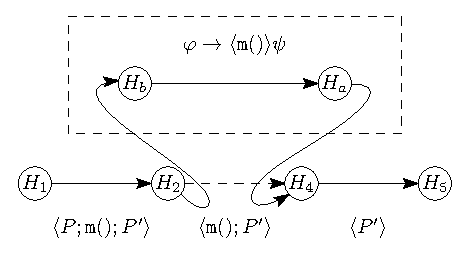
\includegraphics{figures/method_heap.eps}
   \caption{Heaps are `threaded' through method calls. In heap $H_1$ the program fragment $P$ is executed, resulting in heap $H_2$. Either a contract for method \texttt{m()} is employed, which relates the before heap $H_b$ to some heap after the method call $H_a$; or, the method body is unfolded by wrapping it in a method frame that resolves overshadowing of program variables. In both cases, to call the method, heap $H_b$ is equal to $H_2$ and heap $H_a$ is equal to $H_4$. Then the program fragment $P'$ that occurs after the method call is executed using the heap returned by the method.}
   \label{fig:method_heap}
\end{figure}

An important aspect of Java programs are method calls. There are three main issues: calling a method may introduce new program variables that shadow older program variables, calling a method may change the heap, and it is possible to call a method on an object for which its exact type is only known at run-time.

To solve the issue of overshadowing older program variables, KeY uses \emph{method frames}; before a method frame is created, it is ensured that old program variables and new program variables do not collide by renaming the program variables of a method body. Since the \texttt{\textbf{this}} keyword cannot be renamed, the method frame provides a context in which program fragments evaluates \texttt{\textbf{this}} references; it also tracks where the method return value must be placed.

The implicit heap variable is also stored in the method frame, referred to as the before heap. Any heap update within the method is performed on a separate program variable. Statements following a method call are performed using the heap as it is after the method call completes: there are rules for `threading' the heap through a method call, see Figure \ref{fig:method_heap}. There are roughly two ways of treating method calls: unfolding their method body wrapped in a method frame, or using its method contract.

The issue of run-time types is solved using method contracts. Method contracts and other annotations of Java programs are specified in terms of the Java Modeling Language (see~\cite{leavens2013jml}) but with KeY-specific extensions (see \cite[Chapter 7]{KeYbook}). Each method is annotated by a contract that specifies pre- and post-conditions: all implementations of this method should adhere to the contract. The contract determine corresponding correctness formulas in JavaDL: if they are verified, then the corresponding method is correct with respect to its method contract. Consequently, method contracts can be reused in other proofs involving program fragments that call such method.

JML also allows annotations of ghost fields and model fields. Ghost fields are virtual fields that become part of the modelled state of an object on the heap, but are never present when actually executing a Java program. Like normal fields, the value of ghost fields are assigned a default value at object initialization, and can be explicitly changed by JML \texttt{set} annotations. These annotations occur anywhere in method bodies where otherwise a normal statement can be expected. Model fields are introduced as function symbols, and several axioms are added that allow the definition of model fields to be substituted during proof. An example model field is a \emph{class invariant}, which is implicitly assumed to hold of the state of an object between method invocations.

Java programs annotated with JML are entered into the KeY system and the verification begins by generating one or more \emph{proof obligations}. Using the interactive tool, a proof tree is constructed by applying rules until the branches of the tree are closed. Each rule application may result in zero or more branches: in the case of multiple branches, every branch needs to be closed. The tool also provides automation, that automatically applies proof rules using heuristics. This speeds up the verification effort considerably. Finally, after all proof obligations appear as the conclusion of a closed proof tree, the verification effort is done. The proof trees can be stored in a file and reloaded and inspected later.